Идея бустинга: берем несколько последовательных моделей. Каждая следующая предсказывает ошибку предыдущей 

\begin{figure}[H]

\centering

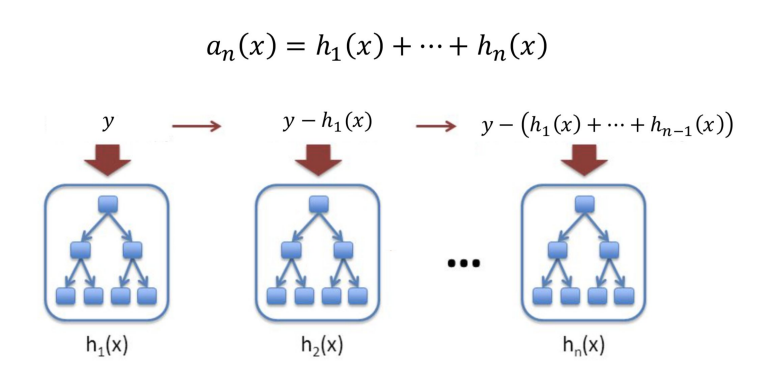
\includegraphics[width=0.8\linewidth]{images/boosting intuition.png}

\end{figure}

\begin{example}
    Рассмотрим игрушечный пример на задаче бинарной классификации (см. картинки ниже). Каждая модель будет <<решающим пнем>> (деревом с одним разделением). После того как обучим все модели с учетом ошибок предыдущих (размер точек показывает ошибку) сложим их с какими-то весами и получим итоговую нелинейную модель
    
    \begin{figure}[H]
    \centering
    \begin{subfigure}
      \centering
      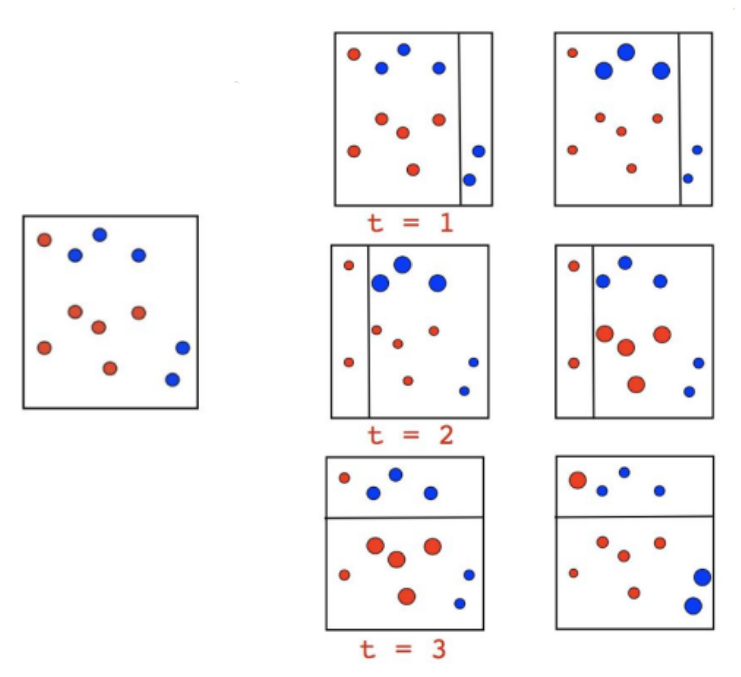
\includegraphics[width=0.4\linewidth]{images/boosting intuition learning.png}
    \end{subfigure}
    \begin{subfigure}
      \centering
      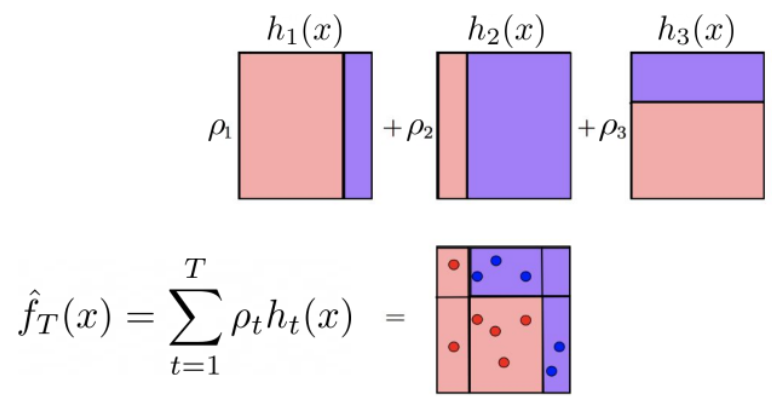
\includegraphics[width=0.4\linewidth]{images/boosting intuition result.png}
    
    \end{subfigure}
    \end{figure}
    
\end{example}

\begin{example}
    Рассмотрим экспоненциальную функцию потерь $E(M)=e^{-M}$. Тогда

    \[ \hat{f}_T = \sum_{t=1}^T \rho_t h_t(x)\]

    \[ L(y_i, \hat{f}_T(x_i)) = \exp (-y_i \hat{f}_T(x_i))=\exp (-y_i \sum_{t=1}^T \rho_t h_t(x_i))=\underbrace{\exp (-y_i \sum_{t=1}^{T-1} \rho_t h_t(x_i))}_{\text{const on step T}} \cdot \exp (-y_i \rho_T h_T(x_i)) =\]
    
    \[=w_i \cdot \exp (-y_i \rho_T h_T(x_i))\]

    Видим, что у каждого объекта есть вес, зависящий от ошибок прошлых моделей, а на шаге $T$ нам нужно минимизирвоать только последнюю функцию. Такой бустинг называется \textit{AdaBoosting} (адаптивный). Однако он был не очень хорош: легко переобучался, экспонента мешала вычислительно и не всегда подходила под задачу
\end{example}

\textbf{Gradient boosting:} идейно мы применяем градиентный спуск в пространстве моделей

Рассмотрим датасет $\{(x_i, y_i)\}_{i=1, \ldots, n}, L(y,f)$ - функция потерь. Тогда оптимальная модель $\hat{f}$ имеет вид

\[ \hat{f}(x)=\argmin_{f(x)} L(y, f(x))=\argmin_{f(x)} \E_{x,y} L(y, f(x))\]

Пусть модель взята из параметрического семейства

\[ \hat{f}(x)=f(x, \hat{\theta})\]

\[ \hat{\theta} = \argmin_\theta \E_{x,y} L(y, f(x, \theta))\]

Рассмотрим шаг индукции: пусть у нас обучены уже $t-1$ последовательных модели. Обозначения:
\[\hat{f}(x) = \sum_{i=0}^{t-1} \hat{f}_i(x)\]

\[ (\rho_t, \theta_t)=\argmin_{\rho, \theta} \E_{x,y} L(y, \hat{f}(x)+\rho \cdot h(x, \theta))\]

\[ \hat{f}_t(x)=\rho_t \cdot h(x, \theta_t)\]

Рассмотрим антиградиент функции ошибки по предсказанию

\[ r_{it} = -\left[ \frac{\partial L(y_i, f(x_i))}{\partial f(x_i)}\right]_{f(x)=\hat{f}(x)}, \quad i=1, \ldots n \]

Настроим нашу следующую модель на предсказание антиградиента

\[ \theta_t = \argmin_\theta \sum_{i=1}^n (r_{it} - h(x_i, \theta))^2 \]

Затем найдем оптимальный шаг в сторону градиента

\[ \rho_t = \argmin_\rho \sum_{i=1}^n L(y_i, \hat{f}(x_i)+\rho \cdot h(x_i, \theta_t)) \]

База индукции: так как каждая следующая модель исправляет ошибку предыдущей нам в принципе неважно с чего начинать, так что можно, например, начать с константы (среднее значение по всему датасету)

Частный случай для линейной регрессии и $L=MSE$

\[ r_{it} = -\left[ \frac{\partial L(y_i, f(x_i))}{\partial f(x_i)}\right]_{f(x)=\hat{f}(x)}=-2(\hat{y}_i - y_i) \]

Получили, что антиградиент пропорционален ошибке, то есть каждая следующая модель напрямую пытается предсказать ошибку предыдущих (в общем случае с другими моделями/функциями потерь это может быть не так)

\begin{lemmanote}
    Важно следить за тем, чтобы градиентный бустинг не переобучился: если переобучится одна модель в цепочке, то все что дальше происходит уже бесполезно. Поэтому если вы пока не понимаете специфику задачи, лучше использовать неглубокие деревья в бустинге (так как их очень сложно переобучить)
\end{lemmanote}

\begin{lemmanote}
    Сам градиентный бустинг не параллелизуется, но так как обычно его делают на деревьев можно распараллелить процесс построения каждого дерева
\end{lemmanote}